\chapter{Bernstein-Vazirani Algorithm}

Now we will discuss the Bernstein-Vazirani problem. It is also called the Fourier sampling problem, although there are more general formulations of this problem that also go by that name.

In order to describe this problem, it will be helpful to introduce some notation. For two binary strings $x = x_{n-1} \ldots x_0$ and $y = y_{n-1} \ldots y_0$, we define
\[
x \cdot y = x_{n-1}y_{n-1} \oplus \ldots \oplus x_0y_0
\]
We'll refer to this operation as the binary dot product. An alternative way to define it is as follows:
\[
x \cdot y = 
\begin{cases} 
1, & \text{if } x_{n-1}y_{n-1} + \ldots + x_0y_0 \text{ is odd} \\
0, & \text{if } x_{n-1}y_{n-1} + \ldots + x_0y_0 \text{ is even}
\end{cases}
\]
Notice that this is a symmetric operation, meaning that the result doesn't change if we swap $x$ and $y$, so we're free to do that whenever it's convenient.

One way to think about the binary product $x \cdot y$ is that it equals the parity of those qubits of $x$ in positions where the string $y$ has a $1$, which is equivalent to the parity of those bits of $y$ in positions where the string $x$ has a $1$.

With this notation in hand, we can now define the Bernstein-Vazirani problem.


\section{The Problem Definition}

\textbf{Input: } A function $f:\{0,1\}^n \rightarrow \{0,1\}$ such that there exists a binary string $s = s_{n-1} \ldots s_0$ for which $f(x) = s \cdot x$ for all $x \in \{0,1\}^n$.\\
\textbf{Output: } The string $s$.

We don't actually need a new algorithm for this problem; the Deutsch-Jozsa algorithm (not including the post-processing step of computing the OR of the measurement outcomes) solves it. In the interest of clarity, let's refer to the quantum circuit above (without the classical post-processing step) the Deutsch-Jozsa circuit given in figure~\ref{fig:deutsch-jozsa}.

\section{The Classical Solution}

While the Deutsch-Jozsa circuit solves the Bernstein-Vazirani problem with a single query, any classical query algorithm must take at least $n$ queries to solve the problem. This can be reasoned through a so-called information-theoretic argument. Each classical query reveals a single bit of information about the solution, and there are $n$ bits of information that need to be uncovered.

It is, in fact, possible to solve the Bernstein-Vazirani problem classically by querying the function on each of the $n$ strings having a single $1$ in each possible position and $0$ for all other bits, which reveals the bits of $s$ one at a time.

So, the advantage of quantum over classical algorithms for this problem is $1$ query versus $n$ queries.



\section{The Quantum Solution: Bernstein-Vazirani Algorithm}

To analyze the Deutsch-Jozsa circuit for the Bernstein-Vazirani problem, we begin with a key observation. Using the binary dot product, we can describe the action of $n$ Hadamard gates on the standard basis state $\ket{x}$ as:
\[
H^{\otimes n}\ket{x} = \frac{1}{\sqrt{2^n}} \sum_{y \in \{0,1\}^n} (-1)^{x \cdot y} \ket{y}
\]
This expression holds because the Hadamard gate introduces a phase of $(-1)^k$ depending on whether $k = x \cdot y$ is even or odd.

Now consider the circuit. Initially, the $(n+1)$-qubit system is in the state $\ket{0}^{\otimes n} \otimes \ket{1}$. After applying Hadamard gates to all qubits, the state becomes:
\[
\left( \frac{1}{\sqrt{2^n}} \sum_{x \in \{0,1\}^n} \ket{x} \right) \otimes \frac{1}{\sqrt{2}} \left( \ket{0} - \ket{1} \right) = \frac{1}{\sqrt{2^n}} \sum_{x \in \{0,1\}^n} \ket{x} \otimes \ket{-}
\]

Next, we apply the oracle $U_f$, defined by $U_f\ket{x}\ket{y} = \ket{x}\ket{y \oplus f(x)}$. Since the second register is in the $\ket{-}$ state, this induces a relative phase based on $f(x)$:
\[
U_f \left( \frac{1}{\sqrt{2^n}} \sum_{x \in \{0,1\}^n} \ket{x} \otimes \ket{-} \right) = \frac{1}{\sqrt{2^n}} \sum_{x \in \{0,1\}^n} (-1)^{f(x)} \ket{x} \otimes \ket{-}
\]

Then, we apply a second layer of Hadamard gates to the first $n$ qubits. Using the earlier identity for $H^{\otimes n}$, the state becomes:
\[
\frac{1}{2^n} \sum_{x \in \{0,1\}^n} \sum_{y \in \{0,1\}^n} (-1)^{f(x) + x \cdot y} \ket{y} \otimes \ket{-}
\]

We're promised that $f(x) = s \cdot x$ for some hidden string $s \in \{0,1\}^n$. Substituting this, the state becomes:
\[
\frac{1}{2^n} \sum_{x \in \{0,1\}^n} \sum_{y \in \{0,1\}^n} (-1)^{s \cdot x + x \cdot y} \ket{y} \otimes \ket{-}
\]

Noting that both $s \cdot x$ and $x \cdot y$ are binary (i.e., in $\{0,1\}$), and that $(-1)^{a + b} = (-1)^{a \oplus b}$ when $a,b \in \{0,1\}$, we rewrite the exponent:
\[
\frac{1}{2^n} \sum_{x \in \{0,1\}^n} \sum_{y \in \{0,1\}^n} (-1)^{(s \cdot x) \oplus (x \cdot y)} \ket{y} \otimes \ket{-}
\]

(Parentheses are used here for clarity. Conventionally, the binary dot product takes precedence over exclusive-OR. This is intuitive, as the dot product behaves like multiplication and XOR like addition.)

To evaluate this, observe that the sum over $x$ collapses unless $y = s$, in which case every term contributes $+1$. Hence, the final state is:
\[
\ket{s} \otimes \ket{-}
\]

Thus, measuring the first $n$ qubits yields the hidden string $s$ with certainty—solving the Bernstein-Vazirani problem using only a single query.


At this point, we'll make use of the following formula:
\[
(s\cdot x)\oplus (y\cdot x) = (s\oplus y)\cdot x
\]
We can obtain this formula through a similar identity for bits:
\[
(ac)\oplus (bc) = (a\oplus b)c
\]
together with an expansion of the binary dot product and bitwise exclusive-OR:
\begin{align*}
    (s\cdot x)\oplus (y\cdot x) &= (s_{n-1}x_{n-1})\oplus \ldots \oplus (s_0x_0) \oplus (y_{n-1}x_{n-1})\oplus \ldots \oplus (y_0x_0)\\
    &= (s_{n-1}\oplus y_{n-1})x_{n-1} \oplus \ldots \oplus (s_0 \oplus y_0)x_0\\
    &= (s\oplus y)\cdot x
\end{align*}

This allows us to express the state of the circuit immediately prior to the measurements as:
\[
\frac{1}{2^n}\sum_{x\in\{0,1\}^n} \sum_{y\in\{0,1\}^n}(-1)^{(s\oplus y)\cdot x} \ket{y}\otimes\ket{-}
\]

The final step is to make use of yet another formula, which holds for every binary string $z = z_{n-1}\ldots z_0$:
\[
\frac{1}{2^n}\sum_{x\in\{0,1\}^n}(-1)^{z\cdot x} =
\begin{cases}
1, &\text{if } z = 0^n \\
0, &\text{if } z \neq 0^n
\end{cases}
\]
(Here, we're using a simple notation for strings: $0^n$ is the all-zero string of length $n$.)

A simple way to argue that this formula works is to consider the two cases separately. If $z = 0^n$, then $z \cdot x = 0$ for every string $x \in \{0,1\}^n$, so the value of each term in the sum is $1$, and we obtain $1$ by summing and dividing by $2^n$. On the other hand, if any one of the bits of $z$ is equal to $1$, then the binary product $z \cdot x$ is equal to $0$ for exactly half of the possible choices for $x \in \{0,1\}^n$ and $1$ for the other half—because the value of the binary dot product $z \cdot x$ flips (from $0$ to $1$ or from $1$ to $0$) if we flip the bit of $x$ in any position where $z$ has a $1$.

If we now apply this formula to simplify the state of the circuit prior to the measurements, we obtain:
\[
\frac{1}{2^n}\sum_{x\in\{0,1\}^n}\sum_{y\in\{0,1\}^n}(-1)^{(s\oplus y)\cdot x}\ket{y}\otimes\ket{-} = \ket{s}\otimes\ket{-}
\]
owing to the fact that $s \oplus y = 0^n$ if and only if $y = s$.

Thus, the measurement reveals precisely the string $s$ we are looking for. The algorithm is summarized in~\ref{algo:bv}.
\begin{algorithm}
    \caption{Bernstein–Vazirani Algorithm}
    \begin{algorithmic}[1]
    \State \textbf{Input:} A black box $U_f$ which performs the transformation $\ket{x}\ket{y} \rightarrow \ket{x}\ket{y \oplus f(x)}$, where $f(x) = s \cdot x \mod 2$, for some hidden string $s \in \{0,1\}^n$.
    \State \textbf{Output:} The hidden string $s$.
    \State \textbf{Runtime:} One evaluation of $U_f$. Always succeeds.
    \State \textbf{Initialize:} An $n+1$ qubit register in the state $\ket{0}^{\otimes n}\ket{1}$.
    \State Apply Hadamard gate to all qubits:
    \[
    \rightarrow \left( \frac{1}{\sqrt{2^n}} \sum_{x\in\{0,1\}^n} \ket{x} \right) \left( \frac{\ket{0} - \ket{1}}{\sqrt{2}} \right)
    \]
    \State Query the oracle $U_f$:
    \[
    \rightarrow \frac{1}{\sqrt{2^n}} \sum_{x\in\{0,1\}^n} (-1)^{f(x)} \ket{x} \left( \frac{\ket{0} - \ket{1}}{\sqrt{2}} \right)
    \]
    \State Apply Hadamard gate to the first $n$ qubits:
    \[
    \rightarrow \frac{1}{\sqrt{2^n}} \sum_{x\in\{0,1\}^n} (-1)^{(s\oplus y) \cdot x} \ket{x} \left( \frac{\ket{0} - \ket{1}}{\sqrt{2}} \right)
    \]
    \State Measure the first $n$ qubits to obtain the bitstring $s$.
    \[
    \rightarrow \ket{s} \left( \frac{\ket{0} - \ket{1}}{\sqrt{2}} \right)
    \]
    \end{algorithmic}
    \label{algo:bv}
\end{algorithm}


\section{Implementation using Qiskit}
\subsection{Background}
Usage estimate: The estimated runtime is approximately 6 seconds; actual runtimes may vary depending on backend load and network conditions.

To run the Bernstein-Vazirani algorithm, we require an oracle that implements the function $f(x) = s \cdot x$ for a secret string $s$ — i.e., a circuit to evaluate it. Here, we demonstrate how to construct such oracles and use gates from the Qiskit Circuit Library to build the circuit. The \texttt{Sampler} primitive in Qiskit Runtime allows for seamless execution of the circuit.

\subsection{Requirements}
Before starting this tutorial, ensure that the following dependencies are installed:
\begin{itemize}
    \item Qiskit SDK 1.0 or later, with visualization support: \texttt{pip install 'qiskit[visualization]'}
    \item Qiskit Runtime (version 0.22 or later): \texttt{pip install qiskit-ibm-runtime}
\end{itemize}

\subsection{Setup}
Here we import the small number of tools needed for this tutorial.

\begin{lstlisting}[language=Python]
#Built-in modules
import math

#imports from Qiskit
from qiskit import QuantumCircuit, QuantumRegister, ClassicalRegister
from qiskit.visualization import plot_distribution
from qiskit_aer import AerSimulator

#Imports from Qiskit Primitives
from qiskit_ibm_runtime import SamplerV2 as Sampler

#Imports from Qiskit Runtime
from qiskit_ibm_runtime import QiskitRuntimeService
\end{lstlisting}

\begin{lstlisting}[language=Python]
# To run on hardware, select the backend with the fewest number of jobs in the queue
# backend = AerSimulator()  # Use AerSimulator for local simulation

# To run on IBM Quantum hardware, uncomment the following lines
service = QiskitRuntimeService(channel="ibm_cloud")
backend = service.least_busy(operational=True, simulator=False)
backend.name
\end{lstlisting}

This will output one of the IBM Quantum computers (e.g., \texttt{ibm\_brisbane}).

\begin{enumerate}
    \item \textbf{Step 1: Map classical inputs to a quantum problem}: \\
    The Bernstein-Vazirani algorithm requires an oracle that implements the function $f(x) = s \cdot x$. Here, we demonstrate how to construct the oracle and use the gates from the Qiskit Circuit Library to easily set up a Bernstein-Vazirani circuit. In this example, we will work with the secret string $s = 1101$.

The runtime Sampler primitive allows seamless execution of the Bernstein-Vazirani circuit.

    \begin{lstlisting}[language=Python]
def berstein_vazirani_circuit(oracle):
    # Create a Quantum Circuit
    qubits=QuantumRegister(oracle.num_qubits,name="q")
    cbits=ClassicalRegister(oracle.num_qubits-1,name="c")
    circuit=QuantumCircuit(qubits,cbits)

    circuit.x(qubits[-1])  # Initialize the last qubit to |1>
    circuit.h(range(oracle.num_qubits))  # Apply Hadamard gates to all qubits
    circuit.append(oracle, qubits)  # Apply the oracle to all but the last qubit
    circuit.h(range(oracle.num_qubits))  # Apply Hadamard gates again to all qubits
    circuit.measure(range(oracle.num_qubits-1), range(oracle.num_qubits-1))  # Measure all qubits
    circuit.name = "Bernstein-Vazirani Circuit"

    return circuit

def build_oracle(s):
    """
    Builds the oracle for the Bernstein-Vazirani algorithm.
    
    Args:
        s (str): A binary string representing the secret string.
        
    Returns:
        QuantumCircuit: The oracle circuit.
    """
    n = len(s)
    oracle = QuantumCircuit(n+1, name='oracle')

    # Apply controlled-X gates based on the secret string
    for i, bit in enumerate(s):
        if bit == '1':
            oracle.cx(i, n)
    
    return oracle
    \end{lstlisting}
   Note that the above code creates an oracle circuit that computes the required function $f(x) = s \cdot x$ with the input string $s$. We now create the Bernstein-Vazirani circuit with the oracle for the secret string $s = 1101$.

    \begin{lstlisting}[language=Python]
s = "1101"
qc = berstein_vazirani_circuit(build_oracle(s))
\end{lstlisting}

Similarly, we can create the oracle for any such secret string.

The circuit, along with the corresponding oracle implementing the function, is shown in Figure~\ref{fig:bernstein_vazirani}.

\begin{figure}[ht]
    \centering
    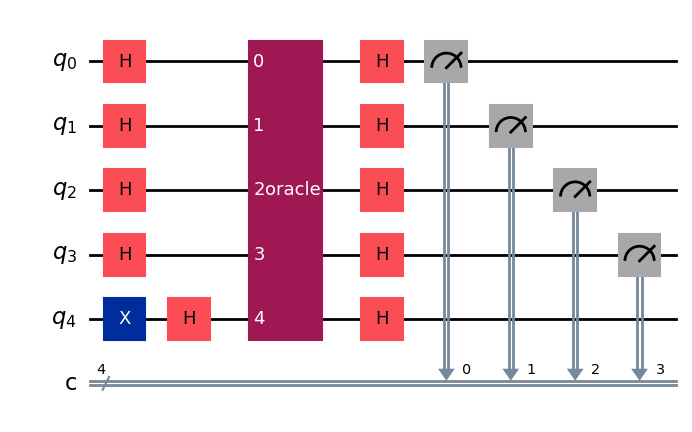
\includegraphics[width=\linewidth]{Images/bernstien-vazirani.png}
    \caption{Bernstein-Vazirani circuit}
    \label{fig:bernstein_vazirani}
\end{figure}

Note that the oracle shown implements the function $f(x) = s \cdot x$ with some secret string $s$.

\item \textbf{Step 2: Optimize problems for quantum execution}
\begin{lstlisting}[language=Python]
from qiskit.transpiler.preset_passmanagers import generate_preset_pass_manager

target=backend.target
pm = generate_preset_pass_manager(backend=backend, optimization_level=3)

circuit_isa_qc=pm.run(qc)
circuit_isa_qc.draw(output="mpl",idle_wires=False,style="iqp")
\end{lstlisting}


\begin{figure}[ht]
    \centering
    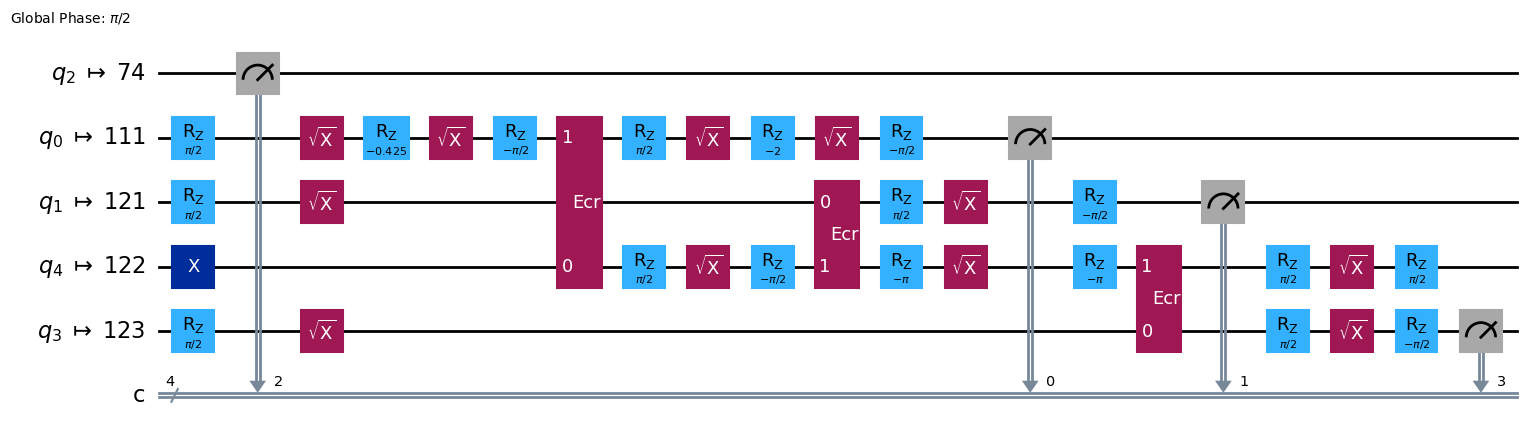
\includegraphics[width=\linewidth]{Images/bv_opt.png}
    \caption{Bernstein-Vazirani transpiled circuit}
    \label{fig:bv_opt}
\end{figure}

The optimized circuit shown in Figure~\ref{fig:bv_opt} is the one that will actually be executed on a quantum computer.

\item \textbf{Step 3: Execute using Qiskit Primitives} \\
We now run the circuit and sample the measurements on the first qubit. For execution, we use the \texttt{Sampler} runtime primitive.

    
    \begin{lstlisting}[language=Python]
# TO run on local simulator:
#1. Use the StatevectorSampler from qiskit.primitves instead
sampler=Sampler(mode=backend)
sampler.options.default_shots=10_000
result = sampler.run([circuit_isa_qc]).result()
dist = result[0].data.c.get_counts()
    \end{lstlisting}
    
    The output of the above code will be a distribution of measurements equal to the size of the secret string.

\item \textbf{Step 4: Post-process results} \\
Now we plot a histogram of the measurements in classical format.

    
    \begin{lstlisting}[language=Python]
from qiskit.visualization import plot_histogram
plot_histogram(dist_const_0)
    \end{lstlisting}
    
    The output of the above code will be a histogram showing the distribution of measurements.

The following output is produced upon running the code on \texttt{ibm\_brisbane}, as shown in Figure~\ref{fig:bv_hist}. The histogram plot is based on 10,000 shots, and the results clearly align with expectations. Minor deviations arise due to the inherent noise in quantum hardware and the probabilistic nature of quantum measurements.

\begin{figure}
    \centering
    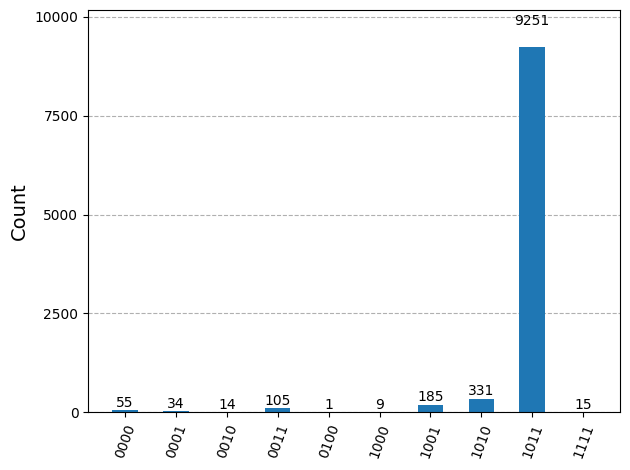
\includegraphics[width=\linewidth]{Images/bv_hist.png}
    \caption{Histogram of measurements}
    \label{fig:bv_hist}
\end{figure}

As seen in Figure~\ref{fig:bv_hist}, the measurement outcome with the maximum occurrence is the string $1011$. Due to the Little Endian convention, this corresponds to the string $s = 1101$ in classical format. This conversion can be done using the following code:
\begin{lstlisting}[language=Python]
# Pick the most frequent outcome
most_frequent_outcome = max(dist, key=dist.get)

# Reverse the bits to get the secret string
secret_string = most_frequent_outcome[::-1]
print(f"The secret string is: {secret_string}")
\end{lstlisting}
This confirms that the secret string is $s = 1101$, as expected. You are encouraged to try this with different secret strings of various lengths.
\end{enumerate}



